\documentclass[10pt,journal]{IEEEtran}

\usepackage{amsmath}
\usepackage{siunitx}
\DeclareSIUnit{\torr}{Torr}
\usepackage{graphicx}
\usepackage{subcaption}
\usepackage{cite}
\graphicspath{{images/}}

\begin{document}

\title{RF Characterization of a Nb-film on a Copper Cavity using a Compact Design}

\author{Andre~R.~Juliao,~Andre~Quintero,~Mehrdad~Kiani,~Lance~Cooley,~and~Shreyas~Balachandran%
\thanks{Manuscript submitted for review to the 2026 Applied Superconductivity Conference.}%
\thanks{A.~R.~Juliao and S.~Balachandran are with the Department of Mechanical and Aerospace Engineering, FAMU-FSU College of Engineering, Tallahassee, FL 32310 USA (e-mail: arj14c@fsu.edu).}%
\thanks{A.~Quintero and L.~Cooley are with the National High Magnetic Field Laboratory, Tallahassee, FL 32310 USA.}%
\thanks{M.~Kiani and S.~Balachandran are with the Department of Materials Science and Engineering, FAMU-FSU College of Engineering, Tallahassee, FL 32310 USA.}%
}

\maketitle

\begin{abstract}

Superconducting films coated on 3D cavities can raise the quality factor of a copper haloscope or accelerator cavity by orders of magnitude. Many superconducting materials and fabrication methods exist, so a robust, rapid method for testing the quality factor of a superconducting film is needed. There are currently many ways to test the RF properties of superconducting films, and here we report the fabrication and 11\,GHz RF characterization of a two-piece hexagonal oxygen-free high-conductivity (OFHC) copper cavity sputter-coated with a \SI{500}{\nano\meter} Ta diffusion barrier and a \SI{700}{\nano\meter} Nb film. The cavity was measured from 2 to \SI{10}{\kelvin} in a Quantum Design Physical Property Measurement System (PPMS), and the unloaded quality factor $Q_0$ was extracted from vector network analyzer $S_{11}$, $S_{22}$, and $S_{21}$ data using a diameter-correction circle fit for the input and output coupling coefficients. For comparison, the bulk Cu cavity was simulated giving $Q_0=77{,}000$ (input $R_s=\SI{5.00}{\milli\ohm}$), and the measured Cu cavity gave $Q_0=62{,}000$, $R_s=\SI{5.65}{\milli\ohm}$, only 19\% below the simulated ideal. The Ta/Nb-coated Cu cavity reached $Q_0 = 1.64\times10^{6}$ at \SI{2}{\kelvin}, corresponding to a surface resistance $R_s = \SI{213}{\micro\ohm}$ (using the simulated geometric factor $G=\SI{350}{\ohm}$). This is roughly 250 times higher than the surface resistance of a comparable niobium cavity at this frequency, indicating that residual resistance dominated. This cavity design allows pre- and post-deposition surface analysis to identify improvements and increase optimization throughput. 
\end{abstract}

\begin{IEEEkeywords}
Niobium thin films, superconducting cavities, quality factor, surface resistance, BCS theory, axion haloscopes.
\end{IEEEkeywords}

\section{Introduction}

3-D resonant cavities with high-quality factors 10$^6$ can be used for dark matter detectors, quantum computers, accelerators, etc. Copper is the ideal cavity body: its high thermal conductivity quickly conducts heat away from hotspot formation in the superconductor, and it can be easily formed to the desired operating frequency. However, the quality factor of Cu saturates to around 10$^4$. If superconducting materials with lower surface resistance, for example Niobium, Nb$_3$Sn, or REBCO, are coated on the inside of a Cu cavity, quality factors can reach ($> 10^5$) in strong magnetic fields (10 T)~\cite{Braine:2024nzi}, or up to 10$^{11}$ at zero magnetic field, as in the case of accelerators ~\cite{Ciovati:2014zti}. 

Nb and NbTi have upper critical fields at or below the fields used in present axion searches, which rules them out of a high-field haloscope on physics grounds alone~\cite{gurevichUseNotUse2011}. Nb$_3$Sn, with $T_c \approx \SI{18.3}{\kelvin}$ and $H_{c2}\approx\SI{30}{\tesla}$, is a leading high-field candidate. The standard route, vapor diffusion of Sn into bulk Nb, gives the highest quality factors reported to date~\cite{posenNb3SnSuperconductingRadiofrequency2017}, but is not compatible with a copper substrate; routes under active development on copper instead include Sn-bronze diffusion~\cite{withanageRapidNbSn2021}, stoichiometric-target magnetron sputtering~\cite{fonnesuRecipeOptimizationSRF2025}, and Nb/Sn co-sputtering~\cite{sayeedFabricationSuperconductingNb3Sn2023}. Complex multilayer Nb$_3$Sn films were prepared but had quality factors that were too low ($< 10^5$) at zero magnetic field. So before committing to a more complex film chemistry, a sputtered Ta/Nb bilayer on the same copper cavity body serves as a control experiment: because Nb is a well-characterized single-element film, its measured performance isolates how much of the achievable $Q$ is already set by the copper substrate, the cavity seam, and the deposition system with a simpler number of dependent variables. This paper reports control measurements on the Cu cavity, and the fabrication and RF characterization of a Ta/Nb-coated two-piece copper cavity, benchmarked against the same body's measured and simulated bare-copper performance and against the BCS-limited surface resistance of niobium.

A further motivation is practical. Most published cavity tests in this field use large-bore superconducting solenoids, \SI{147}{\milli\meter} and \SI{150}{\milli\meter} bores in two recent benchmark results~\cite{posen2023HighQ, alesini2019QUAX}, which leave ample room for thick-walled cavity assemblies. The cavity in this work instead had to fit inside the small sample space of a Quantum Design PPMS, constraining its outer dimension to \SI{26}{\milli\meter}, a factor of six smaller.

This PPMS cavity design was first proposed by Thomas Braine\cite{Braine:2024nzi} and it complements coupon-scale methods used elsewhere in the field for fast recipe characterization, including the SLAC mushroom cavity~\cite{oikawaMushroomCavity2019}, the quadrupole resonator~\cite{luCuBronzeQPR2026}, and the Daresbury choke cavity~\cite{sealChokeCavity2025}. These other coupon methods concentrate the RF field on a flat sample disk rather than a full 3D cavity. Our design shows that coatings can instead be screened on an actual cavity geometry, and that this can be done on a compact, commercially available system used for temperature and magnetic field sweeps.

\section{Cavity Design and Fabrication}

The two-piece hexagonal prism cavity is machined from bulk oxygen-free high-conductivity copper, is \SI{72}{\milli\meter} tall with a \SI{12.25}{\milli\meter} inner wall face length and a minimum wall thickness of \SI{2}{\milli\meter}. The two halves close with four hand-tightened stainless screws and three alignment pegs, operating in the TM$_{010}$ mode near \SI{11}{\giga\hertz}. Each half was mechanically polished by hand with 400 to 1200 grit and electropolished in Phosphoric:butanol (3:2) at 45 C with a stir bar at 600 RPM before deposition.

The RF surface was coated with a \SI{500}{\nano\meter} Ta diffusion barrier by DC magnetron sputtering at \SI{100}{\watt} with a \SI{-100}{\volt} substrate bias in \SI{10}{\milli\torr} Ar at \SI{200}{\celsius}, followed by a \SI{700}{\nano\meter} Nb layer sputtered at \SI{250}{\watt} in \SI{8}{\milli\torr} Ar, also at \SI{200}{\celsius}. After deposition, we hand-polished the mating interface between the two halves to close the seam gap; however, light was still visible when we held the assembled halves up to a light source. Fig.~\ref{fig:cavity} shows the coated cavity halves; the darker Nb film covers the resonating wall, while the interface appears as bare copper due to the post-deposition polish.

\begin{figure}[!t]
    \centering
    
\includegraphics[width=0.85\linewidth]{cavity_photo.png}
    \caption{a) The two-piece hexagonal Cu/Ta/Nb cavity after sputtering the Ta diffusion barrier and Nb film. b) Uncoated Cu found at the joining edge of the hexagon faces.}
    \label{fig:cavity}
\end{figure}

\section{RF Measurement Method}

The assembled cavity was mounted on an RF probe inside a Quantum Design PPMS, enabling temperature control from 2 to \SI{300}{\kelvin} at fields up to \SI{9}{\tesla}; all data reported here were taken at zero applied field. A Keysight PNA vector network analyzer drove the cavity through one antenna (port 1, $S_{11}$) and read out through a second (port 2, $S_{22}$), with transmission recorded as $S_{21}$. The two-piece geometry allows opening the cavity before and after measurement and deposition.

Because both ports were non-negligibly coupled, $Q_0$ was extracted with the diameter-correction circle-fit method rather than assuming weak coupling~\cite{KajfezHwan1984}. For each port, the measured $S_{ii}$ trace was fit to a circle in the complex plane with center offset $C$ and radius $R$; the coupling coefficient follows from
\begin{equation}
d = \frac{2R}{|\Gamma_\text{off}|}, \qquad \beta = \frac{d}{2-d}, \qquad |\Gamma_\text{off}| = |C| + R.
\label{eq:beta}
\end{equation}
Fig.~\ref{fig:qcircle}(a)--(b) shows the resulting fits at \SI{2}{\kelvin}, giving $\beta_1 = 0.53$ at the drive port and $\beta_2 = 0.24$ at the pickup port. The loaded quality factor was obtained from a Lorentzian fit to the normalized transmission $|S_{21}|^2$ [Fig.~\ref{fig:qcircle}(c)], using the 3\,dB bandwidth $\Delta f$ about the resonant frequency $f_0$: $Q_L = f_0/\Delta f = 929{,}000$. The unloaded quality factor then follows from
\begin{equation}
Q_0 = Q_L\left(1+\beta_1+\beta_2\right),
\label{eq:q0}
\end{equation}
giving $Q_0 = 1.64\times10^{6}$ at \SI{2}{\kelvin}.

\begin{figure*}[!t]
    \centering
    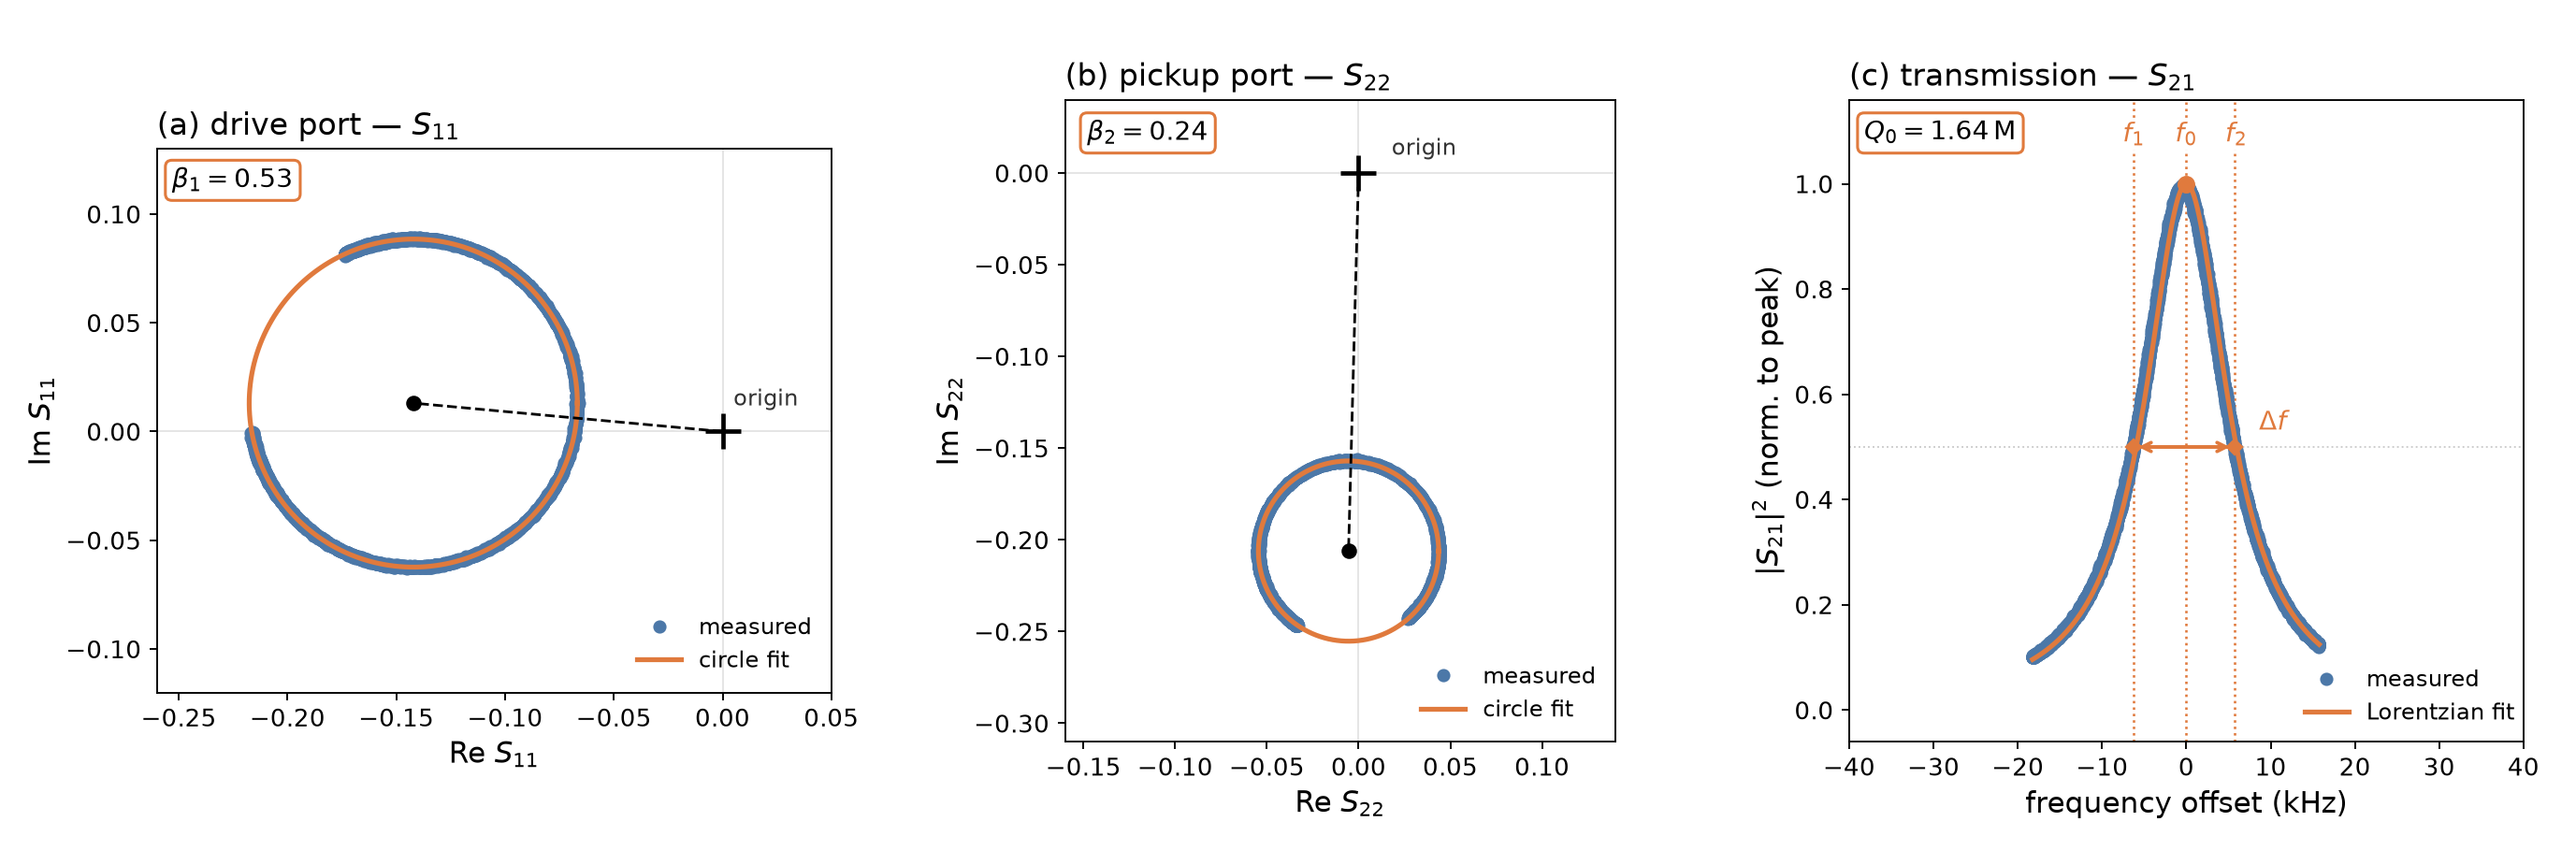
\includegraphics[width=0.95\textwidth]{qcircle.png}
    \caption{Diameter-correction circle fits to the \SI{2}{\kelvin} drive-port (a) and pickup-port (b) reflection data, giving $\beta_1=0.53$ and $\beta_2=0.24$, and the Lorentzian fit to transmission (c) giving $Q_L=929{,}000$. Eq.~\eqref{eq:q0} combines these into $Q_0 = 1.64\times10^{6}$.}
    \label{fig:qcircle}
\end{figure*}

\section{Electromagnetic Simulation}

We modeled the cavity geometry in COMSOL to confirm the TM$_{010}$ mode identity and obtain the geometric factor $G$ used to convert measured $Q$ into surface resistance. Fig.~\ref{fig:sim} shows the simulated electric field for the fundamental TM$_{010}$ mode at $f_0=\SI{11.030}{\giga\hertz}$, together with the two nearest higher-order modes, TM$_{011}$ at \SI{11.395}{\giga\hertz} and TM$_{012}$ at \SI{12.399}{\giga\hertz}. Identifying these modes in simulation was necessary to confirm which resonance mode we were tracking.

From the TM$_{010}$ eigenmode, we computed the geometric factor from the ratio of stored magnetic energy to the surface integral of the tangential magnetic field, giving $G=\SI{350}{\ohm}$ for this cavity. Combined with a literature bulk-copper conductivity, the same simulation gives a simulated bare-copper ceiling of $Q_0=77{,}000$ (input $R_s = \SI{5.00}{\milli\ohm}$), used in Section~V as a cross-check on the measured copper baseline.

\begin{figure}[!t]
    \centering
    
\includegraphics[width=0.95\linewidth]{sim_modes.png}
    \caption{Simulated cavity modes showing electric field volume for a) TM$_{010}$ mode and the two nearest higher-order modes, b) TM$_{011}$ and c) TM$_{012}$. This simulation was used to verify the frequency and geometric factor of the mode, as well as calculate the ideal quality factor of the Cu cavity. The color here is used to show how the mode structure looks with electric field being highest with white and lowest with black and is not to be analyzed quantitatively.}
    \label{fig:sim}
\end{figure}

\section{Results and Discussion}

Fig.~\ref{fig:results} shows the measured surface resistance and unloaded quality factor of the Ta/Nb-coated cavity from 2 to \SI{10}{\kelvin} at zero field, obtained from $R_s = G/Q_0$ at each temperature using the circle-fit procedure of Section~III. We overlay three reference curves: the BCS-limited surface resistance of niobium at \SI{11}{\giga\hertz}, the measured bare-copper baseline of the same cavity body, and the simulated bulk-copper ceiling from Section~IV.

\begin{figure*}[!t]
    \centering
    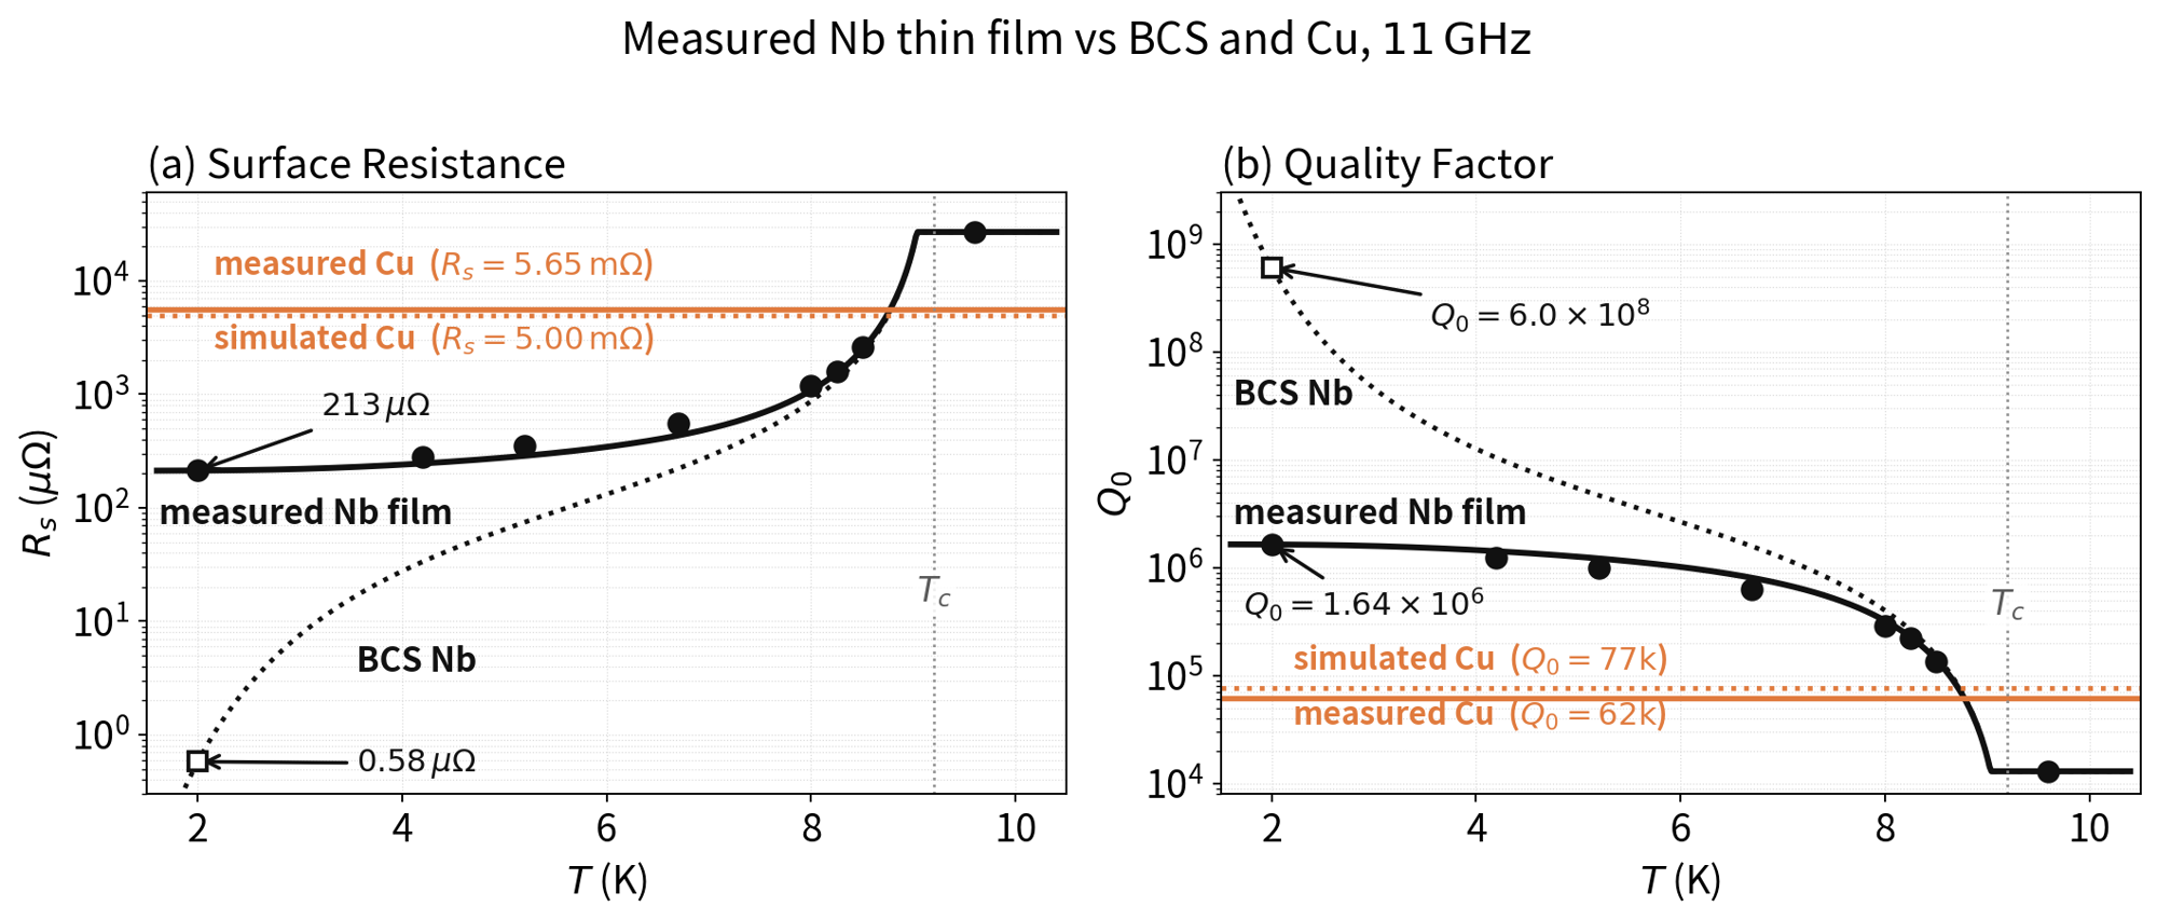
\includegraphics[width=0.85\textwidth]{rs_q0_vs_T.png}
    \caption{Measured surface resistance (a) and unloaded quality factor (b) of the Ta/Nb-coated cavity versus temperature at 11\,GHz and zero field, compared against BCS Nb, the measured bare-Cu baseline, and the simulated bulk-Cu ceiling.}
    \label{fig:results}
\end{figure*}

The measured bare-copper baseline ($Q_0=62{,}000$, $R_s=\SI{5.65}{\milli\ohm}$) is comparable with the independently simulated bulk-Cu ceiling of $Q_0=77{,}000$, confirming that the cavity geometry, fabrication, and measurement method reproduce the expected bulk-Cu performance. Sealing the cavity seam with indium foil raised $Q_0$ from $55,000$ to $62,000$, a simple step we plan to apply to the coated cavity in future work. Against this baseline, the Ta/Nb-coated film reaches $Q_0=1.64\times10^{6}$ and $R_s=\SI{213}{\micro\ohm}$ at \SI{2}{\kelvin}, an improvement of roughly $26\times$. Compared to ideal niobium at this frequency ($R_s \approx \SI{0.58}{\micro\ohm}$ at \SI{2}{\kelvin}, $Q_0\approx 6.0\times10^{8}$), however, our Nb film sits at roughly 250 times higher surface resistance. Surface roughness and uncoated substrate areas are the dominant mechanisms that reduced our quality factor: a Veeco laser-scanning confocal microscope scan of the sputtered Nb surface showed a background roughness of roughly $\pm$\SI{2}{\micro\meter} punctuated by scattered grooves reaching \SIrange{-8}{-11}{\micro\meter}, consistent with polishing scratches that locally disrupted superconductivity. For comparison, electropolished Nb-on-Cu films in the literature reach AFM roughness (Ra) of only \SIrange{6}{21}{\nano\meter}~\cite{Pira2019CuPolish}, two to three orders of magnitude below what is measured here.

Near the superconducting transition, $R_s$ rises gradually before increasing sharply near \SI{8.7}{\kelvin}, slightly below the bulk-Nb critical temperature of \SI{9.2}{\kelvin}. Above $T_c$, $Q_0$ falls to order $10^{4}$. The transition temperature, \SI{.5}{\kelvin} lower than the bulk Nb $T_c$, shows that the superconducting film can be improved, possibly using a thicker layer or HIPIMS~\cite{leithHiPIMSNbCu2023}.

These results add to the growing literature on characterizing the RF properties of superconducting films. We establish a benchmark quality factor with a Nb film. More work is needed to optimize substrate roughness and cavity gap before moving to more complex, higher-$H_{c2}$ coatings such as Nb$_3$Sn.

\section{Conclusion}

We characterized a two-piece hexagonal OFHC copper cavity and compared it to its simulated ideal, finding it about 19\% lower than the ideal. We coated the Cu substrate with a sputtered Ta/Nb bilayer at \SI{11}{\giga\hertz} from 2 to \SI{10}{\kelvin}. The unloaded quality factor of the superconducting film at \SI{2}{\kelvin} was found to be $Q_0=1.64\times10^{6}$ ($R_s=\SI{213}{\micro\ohm}$), roughly $26\times$ better than the cavity's own measured bare-copper baseline. However, we had approximately 250 times the surface resistance of niobium at this frequency (given no extra precaution was taken to reduce flux trapping). Demonstrating this within the small \SI{26}{\milli\meter} bore of a commercial PPMS shows that superconducting thin-film coatings can be screened without dedicated large-bore infrastructure. This measurement establishes a baseline Nb film measurement against which future work with the same design can be compared. This two-piece cavity design allows surface analysis of the sputtered film and quality-factor characterization down to 2K and in high magnetic fields with instruments commonly found in material science labs. 

\section*{Acknowledgment}
This work is supported by the U.S. Department of Energy, Office of Science, Office of High Energy Physics and the Accelerator R\&D and Production (ARDAP) office, under Award No. DE-SC 0018379 and DE-SC0026206. A portion of this work was performed at the National High Magnetic Field Laboratory, which is supported by the National Science Foundation Cooperative Agreement No. DMR-1644779 and the State of Florida.


\begin{thebibliography}{9}

\bibitem{ADMX:2009iij}
S.~J.~Asztalos \emph{et al.}, ``SQUID-based microwave cavity search for dark-matter axions,'' \emph{Phys. Rev. Lett.}, vol.~104, no.~4, p.~041301, 2010.

\bibitem{Braine:2024nzi}
T.~Braine, ``Superconducting resonator development for the Axion Dark Matter eXperiment,'' arXiv:2408.03444 [hep-ex], 2024.

\bibitem{Ciovati:2014zti}
G.~Ciovati, ``AC/RF superconductivity,'' arXiv:1501.07398 [physics.acc-ph], 2014.

\bibitem{gurevichUseNotUse2011}
A.~Gurevich, ``To use or not to use cool superconductors?,'' \emph{Nature Mater.}, vol.~10, no.~4, pp.~255--259, 2011.

\bibitem{posenNb3SnSuperconductingRadiofrequency2017}
S.~Posen and D.~L.~Hall, ``Nb$_3$Sn superconducting radiofrequency cavities: fabrication, results, properties, and prospects,'' \emph{Supercond. Sci. Technol.}, vol.~30, no.~3, p.~033004, 2017.

\bibitem{withanageRapidNbSn2021}
W.~Withanage, A.~Juliao, and L.~Cooley, ``Rapid Nb$_3$Sn film growth by sputtering Nb on hot bronze,'' \emph{Supercond. Sci. Technol.}, vol.~34, 2021.

\bibitem{fonnesuRecipeOptimizationSRF2025}
D.~Fonnesu \emph{et al.}, ``Recipe optimization and SRF test of Cu-compatible Nb$_3$Sn films by DC magnetron sputtering from a stoichiometric target,'' Research Square preprint, 2025.

\bibitem{sayeedFabricationSuperconductingNb3Sn2023}
M.~N.~Sayeed, U.~Pudasaini, G.~V.~Eremeev, and H.~E.~Elsayed-Ali, ``Fabrication of superconducting Nb$_3$Sn film by co-sputtering,'' \emph{Vacuum}, vol.~212, p.~112019, 2023.

\bibitem{posen2023HighQ}
S.~Posen \emph{et al.}, ``High-quality-factor superconducting cavities in Tesla-scale magnetic fields for dark-matter searches,'' \emph{Phys. Rev. Appl.}, vol.~20, p.~034004, 2023.

\bibitem{alesini2019QUAX}
D.~Alesini \emph{et al.}, ``Galactic axions search with a superconducting resonant cavity,'' \emph{Phys. Rev. D}, vol.~99, p.~101101, 2019.

\bibitem{oikawaMushroomCavity2019}
Y.~Oikawa \emph{et al.}, ``Fabrication of Nb mushroom shaped cavity for evaluation of multi-layer thin-film superconductor,'' in \emph{Proc. 29th Linear Accelerator Conf. (LINAC2018)}, 2019, paper TUPO053.

\bibitem{luCuBronzeQPR2026}
M.~Lu \emph{et al.}, ``Preparation of the Cu-based Nb$_3$Sn sample via bronze route for quadrupole resonator testing,'' \emph{Supercond. Sci. Technol.}, 2026, doi: 10.1088/1361-6668/ae496a.

\bibitem{sealChokeCavity2025}
D.~Seal, ``Development of a high throughput facility for the RF characterisation of superconducting thin films,'' Ph.D. dissertation, Lancaster Univ., Dec. 2025.

\bibitem{KajfezHwan1984}
D.~Kajfez and E.~J.~Hwan, ``Q-factor measurement with network analyzer,'' \emph{IEEE Trans. Microw. Theory Tech.}, vol.~MTT-32, no.~7, pp.~666--670, Jul. 1984.

\bibitem{Pira2019CuPolish}
C.~Pira \emph{et al.}, ``Impact of the Cu substrate surface preparation on the morphological, superconductive and RF properties of the Nb superconductive coatings,'' in \emph{Proc. 19th Int. Conf. RF Superconductivity (SRF2019)}, Dresden, Germany, 2019, pp.~935--940.

\bibitem{leithHiPIMSNbCu2023}
S.~Leith \emph{et al.}, ``HiPIMS deposition of superconducting Nb thin films onto Cu substrates,'' \emph{Vacuum}, vol.~212, p.~112041, 2023.

\end{thebibliography}

\end{document}
